% !TEX root = manuscrit.tex

\chapter{Models and Notations}
\label{chap:model}

This chapter introduces the definitions and notations used in the rest of the manuscript. 
We first recall some definitions on graphs and automata that are useful to model the system, 
as well as definitions related to the Linear Temporal Logic, used to express specifications 
of the system. 
We then describe the robot model and its transcription into a product of automata. Finally, we discuss  
implementation issues and we introduce some mechanisms that permit 
to reduce the size of our model.

\section{Background}
Even if several different models have been used to represent
distributed systems \cite{DBLP:books/mk/Lynch96,Tel:2001:IDA:517021,baier_principles_2008}, 
we choose to use a general and
simple one that permits to represent each process of the system, and
its own specificities. 
In particular the system will have global variables; these variables
can be critical resources, or be used as communication channels or
simply be shared data. Each process of the system is represented by a
finite automaton that can access these global variables.  These
automata once combined together represent the system.

\bigskip If $A$ is a finite alphabet, $A^*$ is the set of finite
sequences of elements of $A$ (also called \emph{words}), and
$A^\omega$ is the set of infinite words, with $\varepsilon$ the empty
word. We note $A^+=A^*\setminus \{\varepsilon\}$, and
$A^\infty=A^*\cup A^\omega$. For a word $w\in A^\infty$, we denote its
\emph{length} by $|w|$, with $|w|=+\infty$ for any $w\in
A^\omega$. For two words $w=a_1\cdots a_k\in A^*$, $w'=a'_1\cdots\in
A^\infty$, we define the \emph{concatenation} of $w$ and $w'$ by the
word denoted by $w\cdot w'=a_1\cdots a_ka'_1\cdots$. We usually omit
the dot symbol and simply write $ww'$.  If $L\subseteq A^*$ and
$L'\subseteq A^\infty$, we define $L\cdot L'=\{w\cdot w'\mid w\in L,
w'\in L'\}$.

We denote by $\N$ the set of natural numbers and for any $n \in \N$, we 
use arithmetic modulo $n$, with operations written as $+_n$ (and $-_n$).

 	\subsection{Directed Graphs and automata}
	\label{subsec:automata}\index{Graph}
	A directed graph is a set of vertices connected by directed edges:
	\begin{definition}[Directed graph]
	A directed graph is a pair $G=(V,E)$ where $V$ is a set of vertices
	and $E \subseteq V \times V$.
	\end{definition}
	
	In a directed edge $e = (v_1, v_2) \in E$, 
	$v_2$ is said to be a direct successor of $v_1$, and 
	$v_1$ is said to be a direct predecessor of $v_2$.
	In a directed graph, a path $\pi = v_0v_1\dots \in V^\infty$ is a finite or infinite sequence of vertices  
	such that for all $0< i < |\pi|$,  $(v_{i-1},v_{i}) \in E$.
	
	
	We now recall the classical definition of finite automata. A finite automaton can be seen as a graph with an initial vertex 
	and where edges are equipped with labels.
	
%	\subsection{Automata}
%	\label{subsec:automata}
\index{Automaton}
	\begin{definition}[Finite automaton] 
		A finite automaton $M$  is a tuple
  $(S,s_0,A,T)$ where $S$ is a finite set of states, $s_0 \in
  S$ is the initial state, $A$ is a finite alphabet of actions
  and $T \subseteq S \times (A \cup \{ \varepsilon\}) \times S$
  is a finite set of transitions.
\end{definition} 

A state describes the process at a certain step of its behavior, and
a transition indicates an action that may involve a state change.  A
transition $(s,a,s')$, written $s\xrightarrow{a}s'$, represents a
transition of the automaton from state $s$ to state $s'$ by executing
the action $a$.  The empty word $\varepsilon$ is used as a label to
represent an unobservable (or internal) action.

An execution of $M$ is a sequence of transitions $(s_0,a_1,s_1)$,
$(s_1,a_2,s_2)$, $\dots$ starting in the
initial state $s_0$, written
$s_0\xrightarrow{a_1}s_1\xrightarrow{a_2}\dots$.

For the synchronized product, we introduce a new symbol $-$, denoting
the absence of action for a component. This label implies that the
state of the corresponding component does not change and should not be
confused with a non observable action labeled by $\varepsilon$.
\begin{definition}[Product of automata] 
\label{def:prod} 
  Let $M_1=(S_1,s_{1,0},A_1,T_1)$ and \\
  $M_2=(S_2,s_{2,0},A_2,T_2)$ be two finite automata and let $A$ be an alphabet. 
  A partial synchronization function is a mapping 
  $f:~(A_1 \cup \{\varepsilon, -\})\times(A_2 \cup
  \{\varepsilon, -\})\rightarrow A \cup \{\varepsilon\}$ such that $f(\varepsilon,
  \varepsilon) = f(\varepsilon, -) = f(-, \varepsilon) =\varepsilon$,
  and $f(-,-)$ is undefined.

The product $M=(S,s_0,A,T) = M_1 \otimes_f M_2 $ is defined as
follows: 

\begin{itemize}%[parsep=0cm,itemsep=0cm] 
\item $S = S_1\times S_2 $ is the cartesian product of $S_1$ and $S_2$, 
with $s_0=(s_{1,0},s_{2,0})$ the initial state, 
\item the set $T$ of transitions contains the transition
$(s_1,s_2)\xrightarrow{c}(s'_1,s'_2)$ \textit{iff} 
\begin{itemize}%[parsep=0cm,itemsep=0cm] 
\item there is $(a,b) \in (A_1\cup\{\varepsilon\}) \times
  (A_2 \cup \{\varepsilon\})$ on which $f$ is defined with
  $c=f(a,b)$, and $s_1 \xrightarrow{a} s'_1 \in T_1$, $s_2
  \xrightarrow{b} s'_2 \in T_2,$
\item or there is $a \in A_1\cup\{\varepsilon\}$ such that
  $f(a,-)$ is defined with $c=f(a,-)$, $s_1\xrightarrow{a}s'_1 \in
  T_1$, and $s'_2 = s_2$,
\item or there is $b \in A_2\cup\{\varepsilon\}$ such that
  $f(-,b)$ is defined with $c=f(-,b)$, $s'_1 = s_1$, and
  $s_2\xrightarrow{b}s'_2 \in T_2$.
\end{itemize} 
\end{itemize} 
\end{definition} 

This definition can be easily extended to a set of $n$ automata
$M_1$,~\dots,~$M_n$ with an $n$-ary synchronization function.


	\subsection{Synchronous and asynchronous execution models}
The two extremal cases of synchronized product correspond respectively to totally synchronous and totally asynchronous systems.
% synchro
A synchronous system consists of synchronized rounds of message
exchanges and/or computations.  Hence the synchronization is the most
constrained and the synchronization function $f$ is only defined on
$(A_1\cup\{\varepsilon\}) \times (A_2 \cup \{\varepsilon\})$.

%Asynchro
In a totally asynchronous system the processes can interleave their
steps in an arbitrary order. The corresponding synchronization function is simply
defined on pairs $(a,-)$ or $(-,b)$, when $a \in A_1 \cup
\{\varepsilon\}$, and $b \in A_2 \cup \{\varepsilon\}$ by
$f(a,-)=a$, and $f(-,b)=b$.

%\todo{demon inequitable famine ok mais si un seul veut fire alors il est forcément choisi}

\subsection{Communication}\index{Communication}
 In our model, robots are devoid of any mean of direct communication, 
 the only way for them to communicate is through their observations.
 Robot observation can be seen as a communication by shared variables: 
 when a robot observes the positions of other robots, it reads some informations
 about the other robots and by moving it writes a change of its own information.

Process actions can be divided into three groups: internal events,
reading some variables or writing some variables. When all processes are described by 
automata, the global system will be represented by the product of
these  automata, to which is added a component giving variable valuations.
Hence, the
states are of the form $s=(s_1,s_2, \dots, s_p, V)$, where $s_i$ is
the local state of process $i$, and $V$ is a variable valuation. 
% For the initial state $s_0$ initial valuation for all variables is given.

A transition of the system is of the form $(s_1, \dots, s_p,V)
\xrightarrow{a} (s_1',\dots,s_p',V')$ where $a=f(a_1, \dots,a_p)$ is
simply denoted by the tuple $(a_1, \dots,a_p)$ and defined for $a_i
\in A_i\cup\{\varepsilon,-\}$, $1\leq i \leq p$, if and only if for
any $(i,j)$ such that $i \neq j$, $a_i$ and $a_j$ do not access the
same variables.



\section{\textsf{LTL} specifications}\index{LTL}
\label{def:LTL}
	\subsection{Notations}
	Given a set $\mathcal{P}$ of atomic propositions, the
temporal logic \textsf{LTL} (for Linear Temporal Logic) is a
specification language interpreted on infinite sequences over
$2^{\mathcal{P}}$.  The \textsf{LTL} formulae are defined by the
following grammar:\label{LTL}
\[\varphi::=~p~|~\varphi_1\vee\varphi_2~|~\neg\varphi~|~\X\varphi~|
~\varphi_1 \U \varphi_2\]
where $p \in \mathcal{P}$, $\vee$ is the boolean disjunction, $\neg$
is the negation, and $\X$ (next) and $\U$ (until) are temporal
operators described below.
Moreover two temporal operators $\F$ and $\G$ are usually defined from
$\U$ by: $\F\varphi = \true \U \varphi$ (where $\true$ is an abbreviation of 
$p \vee \neg p$) and 
$\G\varphi=\neg\F\neg\varphi$. The formula $\F\varphi$ states that
$\varphi$ holds \emph{eventually}, and $\G\varphi$ is satisfied
$\textit{iff } \varphi$ holds \emph{forever} from now on.
Temporal and boolean operators can be nested. For instance
$\Diamond\Box\varphi$ expresses that from some position in the future
$\varphi$ always holds, and $\Box\Diamond\varphi$ states that
$\varphi$ is satisfied infinitely often.

For $w \in (2^{\mathcal{P}})^\omega$, written $w=w_1 w_2, \dots$ with
$w_i \in 2^{\mathcal{P}}$, we note $w,i \vDash \varphi$ when $\varphi$
is satisfied at position $i$ of $w$ (\ie from $w_i$ on).
The satisfaction relation is defined inductively by the rules given in
Table~\ref{table}.
 \begin{table}[h!] 
 \center
 \begin{tabular}{ll} 
 $w, i \vDash p$ &$\textit{iff } \ p \in w_i$\\ 
 $w, i \vDash \neg \varphi$ &$\textit{iff } \ w, i \nvDash \varphi$\\ 
 $w, i \vDash \varphi_1 \vee \varphi_2$ & $\textit{iff } \ w, i \vDash 
\varphi_1$ or $ \ w, i \vDash \varphi_2$\\ 
 $w, i \vDash \X\varphi$ &$\textit{iff } \ w, i+1 \vDash \varphi$\\ 
 $w, i \vDash \varphi_1\U\varphi_2$ &$ \textit{iff } \ \exists j \geq i 
\mid w, j \vDash \varphi_2 \text{ and }\forall i \leq k < j, \ w,k \vDash \varphi_1$
\end{tabular} 
\caption{\textsf{LTL} satisfaction relation.} \label{table}
\end{table}

\smallskip To interpret \textsf{LTL} formulae on executions of an
automaton $M~=~(S,s_0,A,T)$, the transition relation is assumed to be
\emph{non blocking}: for each $s \in S$, there is at least one
transition starting from $s$.  Moreover, a labeling function
$\mathcal{L}: S \rightarrow 2^{\mathcal{P}}$ is added to $M$. This
function maps each state of $M$ to a set of atomic propositions that
hold in this state.
With execution $e: s_0 \xrightarrow{a_1} s_1 \xrightarrow{a_2} s_2
\xrightarrow{a_3} \ldots$ of $M$, we associate the infinite word 
$w = \mathcal{L}(s_0) \mathcal{L}(s_1), \dots$. 
For formula $\varphi$, we note $e, i \vDash \varphi$ if $w,i \vDash \varphi$. 

\begin{definition} An automaton $M$, with labeling $\mathcal{L}$,
  satisfies $\varphi$ if for each execution $e$ of $M$, $e, 0 \vDash
  \varphi$.
\end{definition}

Given an automaton $M$ that represents all possible behaviors of a
system and an \textsf{LTL} formula $\varphi$ describing a requirement
on the system, \textsf{LTL} model-checking answers the question
whether $M \models \varphi$ or not.
When the answer is negative, a counter-example can be exhibited.

\subsection{Fairness}\index{Fairness}
For our purpose, correctness of the algorithms must be satisfied with a fair scheduler.
Therefore, only fair executions of the system are considered. To express fairness properties in \textsf{LTL},
we consider two propositions associated with a process $p$: $\textit{enabled}_p$ describes a state of process $p$ 
where at least one action is enabled and $\textit{executed}_p$ corresponds to a state where $p$ is scheduled. 
\begin{description}
\item [Strong Fairness]
For all processes $p$: $(\G\F \textit{enabled}_p) \implies (\G\F \textit{executed}_p)$.
\item[Weak Fairness]
For all processes $p$: $(\F\G\textit{enabled}_p) \implies (\G\F\textit{executed}_p)$.
\item[Unconditional fairness]
For all processes $p$: $\G\F\textit{executed}_p$.
\end{description}
In order to verify a property $\varphi$ only on fair executions of the system
modeled by $M$, we in fact verify $M \models (\textit{fair} \implies \varphi)$.
In the sequel fairness means unconditional fairness.


\section{Model for the robot algorithms}
%	\subsection{Modeling}
In the sequel we are interested in systems where 
all robots execute the same algorithm~\cite{FPS12}, hence the
 behavior of each of them can be described by the same finite automaton. 
We first explain how this automaton describes the robot behavior. We then 
 introduce a scheduler model that permits to obtain different execution models
 by representing the synchronization function by automata. The system is finally 
 obtained by synchronizing robots with the scheduler, and we discuss 
 implementation of the model with respect to  the input language of specific tools.
 
  
		\subsection{Robot Modeling}
 \label{sec:mod:robots}  
 Robots operate in \emph{Look}, \emph{Compute}, and
 \emph{Move} \emph{cycles} that can be seen in the automaton of
 Figure~\ref{fig:1}. \index{Look-Compute-Move}
\begin{figure}[htbp] 
\centering 
\begin{tikzpicture} [thick, node
distance= 10em,>=stealth,->, scale=0.8, transform shape] 
\node[ellipse, minimum height=3em,minimum width= 6em, draw](a) {};
\node[text width=4em, text centered] (a1) []{Ready to look};
\node[ellipse, minimum height=3em,minimum width= 7em, draw,right of=a](b){};
\node[text width=4em, text centered, right of=a] (b1)[]{Ready to compute}; 
\node[ellipse, minimum height=3em,minimum width= 6em,draw,right of=b](c){};
\node[text width=4em, text centered] (c1) [right of=b]{Ready to move};
\node (init) [below left = 1em and 2em of a, node distance= 5em] {};

\path (a) edge[] node[above]{\Look} (b) 
(b) edge[] node[above]{\textit{Compute}} (c) 
(c) edge[bend left] node[above]{\Move}
(a) (init) edge[] node{} (a);

\end{tikzpicture}
\caption{A generic automaton for the robot behavior.} 
\label{fig:1}
\end{figure}

To start a cycle, a robot takes a snapshot of its environment which is
represented by the $\Look$ transition. Then, it computes its
future location, represented by the $\textit{Compute}$
transition. Finally the robot moves according to its previous 
computation, this effective movement is represented by 
the $\Move$ transition.

In the sequel we work on the discrete environment represented by a graph,
where nodes represent locations, and edges represent the possibility 
for a robot to move from one location to the other. 


The algorithm is implemented in the \emph{Compute} transition, hence
the ``Ready to move'' state is divided into as many parts as there are
possible movements according to the protocol under study and the 
graph topology.
 

Note that the original model abstracts the precise time constraints (like 
the computational power or the locomotion speed of robots) and keeps
only sequences of instantaneous actions, assuming that each robot 
completes each cycle in finite time. The model can be reduced by combining
the $\Look$ and $\textit{Compute}$ phases to obtain the $\LC$
phase. This is simply done by merging the two states ``Ready to look''
and ``Ready to compute'' into a single state ``Ready to Look-Compute'' noted $\textit{RLC}$.

To ensure the progress of the protocols, an implicit \emph{fairness}
assumption states that all robots must be infinitely often scheduled,
which is expressed in \textsf{LTL} by: \[\emph{Fairness}:\index{Fairness}
\bigwedge\limits_{i=1}^k \G\F\big(RM_i\big)~\wedge~
\bigwedge\limits_{i=1}^k \G\F\big(RLC_i\big)\] where $RM_i$
(respectively $RLC_i$) is the label corresponding to one of the states
``Ready to Move'' (resp. to the state ``Ready to Look-Compute'') of
robot $r_i$.



\subsection{Scheduler Modeling} 
\label{sec:mod:schedulers} The scheduler organizes robot movements to
obtain all possible behaviors with respect to the execution model,
%Fsync (Fully Synchronous), Ssync (Semi Synchronous) or Async (Asynchronoous)
which depends on the synchronization hypotheses and defines 
the particular synchronization function.
As the robots it is modeled by a finite automaton, one
for each variant of the execution model, but unlike robots that 
have the same behavior regardless of the model, the scheduler 
is parameterized by the number of robots. By synchronizing one of these
schedulers with robot automata, we obtain an automaton that represents
the global behavior of robots in the chosen model.  

To describe these scheduler models, we consider a set
$\Rob=\{r_1, \ldots, r_k\}$ of $k$ robots. We denote by
$\LC_i$ (respectively $\Move_i$), the $\LC$
(resp. $\Move$) phase of robot $r_i$. Note that
$\LC_i$ and $\Move_i$ are actually sets of possible
actions in the corresponding phases. For a subset
$\Sched\subseteq\Rob$, we denote the synchronization
of all $\LC_i$ (respectively $\Move_i$) actions of all
robots in $\Sched$ by:\\ $\prod\limits_{r_i \in
  \Sched}\LC_i$ (respectively $\prod\limits_{r_i \in
  \Sched}\Move_i$).
  
  
  The particular execution models are: Fsync (Fully Synchronous), Ssync (Semi Synchronous)
  or Async (Asynchronous). We describe each of them in the sequel.

In the Ssync\index{Ssync} model, a non-empty subset of robots is scheduled for
execution at every phase, by choosing first a subset $\Sched$ of $\Rob$, and operations are executed
synchronously. In this case, the automaton is a cycle, where a set
$\Sched \subseteq \Rob$ is first chosen. In this cycle
the $\LC$ and $\Move$ phases are synchronized for this set
of robots. A generic automaton for Ssync is described in
Figure~\ref{fig:schedSYm}.  Actually, the ``$\Sched$ chosen''
state has to be divided into $2^k-1$ states, where $k$ is the number of
robots, in order to represent all possible sets $\Sched$.

The Fsync model is a particular case of the Ssync model, where all
robots are scheduled for execution at every phase, and operate
synchronously thereafter:  
In each global cycle, $\Sched = \Rob$, hence all
global cycles are identical.

\begin{figure*}[htbp] 
\centering
\subfloat[) Ssync model.]{
	\centering
		\begin{tikzpicture}[thick, node distance= 11em,>=stealth,->, scale=0.75, transform shape]
	\node[ellipse, minimum height=3em,minimum width= 5em, draw](a){};
	\node[text width=4em, text centered] (a1){$\Move$ Done}; 
	\node[ellipse, minimum height=3em,minimum width= 5em, draw, right of=a](b){};
	\node[text width=4em, text centered] (b1) at(b){$\Sched$ chosen}; 
	\node[ellipse, minimum height=3em,minimum width= 5em, draw, right of = b](c){};
	\node[text width=4em, text centered] (c1) at(c){$\LC$ Done}; 
	\node (init) [below left of=a, node distance= 5em] {};
	
	\path 	(a) edge[] node[above]{$\mathit{Choose~Sched}$} (b) 
			(b) edge[] node[above]{${\prod\limits_{i \in \Sched}} LC_i $} (c) 
			(c) edge[bend left] node[below]{${\prod\limits_{i \in \Sched}} \Move_i $} (a)
			(init) edge[] node{} (a); 
	\end{tikzpicture} 
	\label{fig:schedSYm} 
} 
%\hspace{1em}
\subfloat[) Async model.]{
\centering
	\begin{tikzpicture}[thick, node distance= 14em,>=stealth,->, scale=0.75,transform shape] 
	\node[ellipse, minimum height=3em,minimum width= 5.5em, draw](a2){};
	\node[text width=4em, text centered] (a21) at(a2){\textit{Act} Done}; 
	\node[ellipse, minimum height=3em,minimum width= 5em, draw, right of = a2](c2){};
	\node[text width=4em, text centered] (c21) at(c2){$\Sched$ chosen}; 
	\node (init) [below left of=a2, node distance=5em] {};

	\path	(a2) edge[bend left] node[above]{Choose $\Sched$} (c2)
			(c2) edge[bend left] node[below]{${\prod\limits_{i \in \Sched}}\mathit{Act}_i $} (a2) 
			(init) edge[] node{} (a2); 
	\end{tikzpicture}
	\label{fig:schedCORDA} 
}
\caption{Scheduler automata.} 
\label{essai}
 \end{figure*} 
 The scheduler for the Async\index{Async} model is the one representing 
a totally asynchronous synchronization function.
Any finite delay may elapse
 between $\LC$ and $\Move$ phases: During each phase a
 set $\Sched$ is chosen, and all robots in this set execute an
 action: the action $\textit{Act}_i$ is either in $\LC_i$ or
 in $\Move_i$ depending on the current state of robot
 $r_i$. Hence, a robot can move according to an outdated
 observation. The automaton for this scheduler is depicted in
 Figure~\ref{fig:schedCORDA}.

 \subsection{System Modeling} \label{sec:mod:composition} 
 %%%%%%%%%%% Configuration definition %%%%%%%
 A configuration $c$ of the system describes robot positions on the graph.  
 A node of this graph is called a position, and the set of positions 
 is denoted by $\Pos = \{0,\dots,n-1\} \subseteq \N$.
 A configuration is a mapping $c: \Rob \rightarrow \Pos$
 associating with each robot $r$ its position $c(r) \in
 \Pos$. Hence, in a graph of $n$ nodes with $k$ robots there
 are $n^k$ possible configurations.
 Let $\Config$ be the set of all possible configurations of the system.
 
 The model of the system is an automaton $M =(S, s_0, A, T)$ obtained
 by the synchronized product of $k$ robot automata and all the
 possible configurations, as defined above (Section~\ref{subsec:automata}), 
 where the scheduler is used to define the synchronization function. The
 alphabet of actions is $A = {\prod_{r_i \in \Rob}}\
 \textit{A}_i$, with $A_i = \LC_i \cup \Move_i$ for
 each robot $r_i$. In the resulting automaton, states, also called system states in the sequel, are of the form $s =
 (s_1,\dots,s_k,c)$ where $s_i$ is the local state of robot $r_i$, and
 $c$ the configuration. An initial state is of the form
 $s_0=(s_{1,0},\dots,s_{k,0},c)$ where $s_{i,0}$ is the initial local
 state of robot $r_i$ and $c\in \Config$ is an arbitrary configuration.

 A transition of the system is labeled by a tuple $a=(a_1, \ldots,
 a_k)$, where $a_i \in A_i \cup \{\varepsilon, -\}$ for all $1 \leq i
 \leq k$ and $(s_1,\dots,s_k,c) \xrightarrow{a} (s'_1,\dots,s'_k,c')$
 if and only if for all $i$, $s_i \xrightarrow{a_i} s_i'$ and $c'$ is
 obtained from $c$ by updating the positions of all robots such that
 $a_i \in \Move_i$. Note that when $a_i \in \textit{LC}_i$, the configuration is not modified.
 To represent the scheduling, we denote by
 ${\prod_{r_i \in \Sched}} \textit{Act}_i$ the action $(a_1,
 \ldots, a_k)$ such that $a_i = -$ if $r_i \notin Sched$ and $a_i \in
 \LC_i \cup \Move_i \cup \{\varepsilon\}$ otherwise.
 
 
 
 		\subsection{Implementation issues} 
		\label{sec:mod:divine} 
For our verification purpose, we consider two model-checkers:
DiVinE~\cite{Divine13} and ITS-tools~\cite{LIP69510}. We
chose these model-checkers for their ability to deal with large models
and formulae, by using parallel computations for the first one or a
symbolic approach for the second one. Moreover, both tools provide
several metrics such as the number of states and transitions and they
can handle the same input files.  In particular, the original modeling
language of DiVinE is DVE, which is also interpreted by ITS-tools.  A
DVE system is composed of processes, that are automata where
transitions can be guarded by a \emph{condition} (or \emph{guard})
that determines if the transition can be fired. Therefore, the
transcription of algorithms in DVE is straightforward.

In general, protocols in Fsync, Ssync, or Async models are described
as a set of guarded actions. 
A guard of a robot algorithm is a guard on a $\LC$ transition.
Transitions have so-called \emph{effects} that actually are
assignments to local or global variables. These correspond to the
actions of a guarded-action algorithm. When two transitions can be
fired, one of them is chosen nondeterministically.

\smallskip Although the DiVinE language has a large expressive power,
we had to deal with an important restriction: The DVE language cannot
synchronize more than two automata. Therefore, we implement
synchronized actions using a sequential order such that look/compute
actions ($\LC_i$) are executed first, and the move actions
($\Move_i $) afterward.

More formally, we obtain the following system: $M' =(S', S_0, A, T')$
where $S'$ is defined similarly to $S$, with the addition of a
labeling of states (explained below), to indicate if the state is a
transient or a steady state.  The transition relation is defined as
follows: Any transition $s \xrightarrow{a} s'$ in $M$ is replaced in
$M'$ by a sequence of transitions, where all intermediate states are
labeled as transient, while $s$ and $s'$ are steady states. More
precisely, we note $\hat{a}_i=(-, \ldots, -, a_i, -,\ldots, -)$ the
tuple of actions where only the robot $r_i$ executes $a_i \in A_i$.
An action $a={\prod_{r_i \in \Sched}} \textit{Act}_i$ is
executed as the sequence of actions $\hat{\ell}_1, \ldots,
\hat{\ell}_k, \hat{m}_1, \ldots, \hat{m}_k$ where $\ell_i \in
\LC_i$ if $Act_i \in \LC_i$ and $-$ otherwise, and
similarly, $m_i \in \Move_i$ if $Act_i \in \Move_i$
and $-$ otherwise. Note that for each $i$, $\hat{\ell}_i$ and
$\hat{m}_i$ are either $(-, \ldots,-)$ (containing only $-$, which
corresponds to no action from any robot), or belong to $\{\hat{Act}_i
\mid r_i \in \Sched \}$.

Let $\textit{Exec}(M)$ and $\textit{Exec}(M')$ be respectively the set
of executions of $M$ and $M'$. We denote by $\textit{cf}(e)$ the
sequence of configurations in $e \in \textit{Exec}(M)$ and by
$\textit{cfs}(e')$ the sequence of configurations of the steady states
in $e' \in \textit{Exec}(M')$. This notation is extended to the set of
executions of $M$ and $M'$ by:
$$\textit{cf}(\textit{Exec}(M)) =
\{\textit{cf}(e), e \in \textit{Exec}(M)\},$$
$$\textit{cfs}(\textit{Exec}(M')) = \{\textit{cfs}(e), e \in
\textit{Exec}(M')\}.$$
We say that two executions $e \in Exec(M)$ and
$e' \in Exec(M')$ are equivalent if $\textit{cf}(e)=\textit{cfs}(e')$.

\begin{definition}[Model equivalence] The models $M$ and $M'$ are equivalent if
  $$\textit{cf}(\textit{Exec}(M))=\textit{cfs}(\textit{Exec}(M')).$$
\end{definition}

The following theorem states that our implementation is equivalent to
the abstract asynchronous model (see Figure~\ref{fig:schedCORDA}).
\begin{theorem} The DiVinE implementation is equivalent to the
  abstract Async model.
\end{theorem}

\begin{proof} Let $M$ be the abstract Async model and $M'$ the model
  obtained from $M$ as described above. Since $M$ contains all possible executions of the system,
  we clearly have $\textit{cfs}(\textit{Exec}(M')) \subseteq
  \textit{cf}(\textit{Exec}(M))$. To obtain the converse inclusion, we
  must prove that for each execution $e \in \textit{Exec}(M)$ we can
  find an execution $e' \in \textit{Exec}(M')$ such that $e$ and $e'$
  are equivalent.  This amounts to proving that $M'$ simulates $M$ for a
  simulation relation linking a state of $M$ with the corresponding
  steady state of $M'$, as well as with all the consecutive transient
  states.


  Let $e \in \textit{Exec}(M)$. With any transition $t: s
  \xrightarrow{a} s'$ in $e$, with $a=(a_1, \ldots, a_k)$, we
  associate the execution $e_t$ in $M'$ defined above by: $$s
  \xrightarrow{\hat{\ell}_1} s_1 \ldots \xrightarrow{\hat{\ell}_k} s_k
  \xrightarrow{\hat{m}_1} s'_1 \ldots \xrightarrow{\hat{m}_k} s'_k$$
  with all look actions before all move actions.  We now define the
  execution $e' \in M'$ by replacing all transitions $t$ in $e$ by
  $e_t$. We must now prove that $e$ and $e'$ are equivalent.

  For this, we show that each transition $t: s \xrightarrow{a} s'$ is
  equivalent to $e_t$ by examining the ordering of actions. We say
  that two actions $\hat{a}_i$ and $\hat{a}_j$ commute, 
  if for any system state $p$, if
  $r\xrightarrow{a_i} p_1 \xrightarrow{a_j} p'$, there exists $p'_1$
  such that $p \xrightarrow{a_j} p'_1 \xrightarrow{a_i} p'$. This
  expresses the fact that the state reached is independent of the
  order of actions $\hat{a}_i$ and $\hat{a}_j$. Clearly, any two
  $\LC$ actions commute since they only modify the local state
  of the robot they belong to, and only depend on the current
  configuration that is not updated by $\LC_i$. Similarly, any two
  $\Move$ actions on different robots commute, since they
  successively update the positions of robots $i$ and $j$ in
  $c$. Moreover, from the definition of $M$, all actions $\hat{a}_i$
  being simultaneous, the $\LC$ actions must observe the
  initial configuration $c$ in the initial steady state
  $s$. Therefore, since all $\LC$ actions appear before the
  move actions in $e_t$, this (sequential) execution is equivalent to
  the (simultaneous) version $t$. Combining all transitions in $e'$,
  we obtain that $e'$ and $e$ are equivalent, which concludes the
  proof.
\end{proof}
		
\section{Methodology for the ring}
We denote by $\Pos=\{0,\dots, n-1\}  \subseteq \N$ the set of positions on a ring of size $n$. 
Note that node $i\plusN 1$ is the successor of node $i$ in the clockwise direction.

\subsection{Configurations} %configurations défini dans  \ref{sec:mod:composition}
\label{subsubsec:conf}
\index{Configuration}
Since robots and nodes are anonymous, we gather the different configurations in 
an equivalence class such that only relative positions of the robots are taken into account.
In the sequel we denote by $\circ$ the composition of applications, and by $id$ the identity function.
 
Let $\pi$ and $\overline{\pi}$ be the permutations of
$\Pos$ defined as follows:
\begin{itemize}
\item $\pi(i)=i \plusN 1$ for $i \in \Pos$, $\pi^0=id$ and $\pi^{m+1}= \pi \circ \pi^m$ for any $m \in \N$. 
\item $\overline{\pi}(i) = n \moinsN i$ for $i \in \Pos$.
\end{itemize}
 The first permutation corresponds to a one step shift in the
clockwise direction, while the second one is an axial symmetry with
respect to the diameter of the ring containing node $0$. 
Hence $\overline{\pi}^2= \pi^n=id$, so that
$\overline{\pi}^{-1} = \overline{\pi}$, and we denote by
$\pi^{-m}$ the inverse of $\pi^{m}$.

\begin{definition}[Configuration equivalence]
\label{def:confEq}
The equivalence relation $\Cequiv$ on the set $\Pos^{\Rob}$ of
configurations is defined for configurations $c$ and $c'$ by: $c
\Cequiv c'$ if there exists an integer $m$ and some permutation $\beta$
of $\Rob$ such that $c' = \pi^m \circ c \circ \beta$ or
$c'= \overline{\pi} \circ \pi^m \circ c \circ
\beta$.
\end{definition}

\begin{example}
\label{ex:confEq}
All configurations in Figure \ref{fig:confEq} are equivalent.\\
Configuration $a$: $a(r_1) = 2$, $a(r_2) = 4$, $a(r_3) = 7$, $a(r_4)=4$
is equivalent to configuration $b$: $b(r_1) = 4$, $b(r_2) = 6$, $b(r_3) = 9$, $b(r_4)=6$
since $b = \pi^{-2} \circ a$.\\
Configuration $b$ is equivalent to configuration $c$: $c(r_1) = 8$, $c(r_2) = 6$, $c(r_3) = 3$, $c(r_4)=6$.
We have $c = \overline\pi \circ b$ and $b = \pi^{-2} \circ a$, thus $c = \overline\pi \circ \pi^{-2} \circ a$.\\
Configuration $c$ is equivalent to configuration $d$: $d(r_1) = 3$, $d(r_2) = 6$, $d(r_3) = 8$, $d(r_4)=6$.
Let $\beta$ be the permutation defined by: $\beta(r_1) = r_3$, $\beta(r_2)=r_2$, $\beta(r_3)=r_1$, and $\beta(r_4)=r_4$. We have $d = c \circ \beta$, hence we have $d = \overline\pi \circ b \circ \beta $ and $d =\overline\pi \circ \pi^{-2} \circ a \circ \beta$.
\begin{figure}[htbp]
	\subfloat[][
	]{
			\centering 
			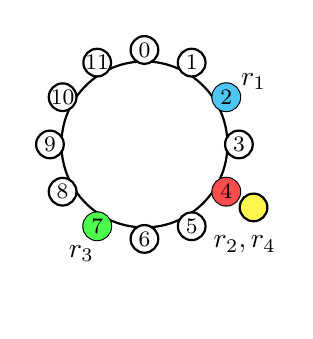
\begin{tikzpicture}[node distance =15em,>=stealth,->, thick] 
			\node[circle,minimum size =6em, draw, thick] (C){};
			\foreach \i in {0,...,11}\node[circle,minimum size
			=1em,draw,fill=white,thick]at(\i*30:1.2) (\i){};
			\node[circle,minimum size =1em,fill=cyan!70]at(1*30:1.2) (17){};
			\node[]at(1*30:1.6) (1721){{$r_1$}};
			\node[circle,minimum size =1em,fill=red!70]at(11*30:1.2) (18){}; 
			\node[circle,minimum size =1em,fill=yellow!70,draw,thick]at(11*30:1.6) (18){}; 
			\node[]at(10.5*30:1.8) (181){{$r_2,r_4$}}; 
			\node[circle,minimum size =1em,fill=green!70]at(8*30:1.2) (29){};
			\node[]at(8*30:1.6) (191){{$r_3$}}; 
			
			\foreach \i in {0,...,11}\node[circle,minimum size
			=1em]at(90 - \i*30:1.2) (pos){\footnotesize{\i}};
			
			\node[]at(9*30:2) (181){\large{$~$}}; 

			\end{tikzpicture}
	}\hspace{-1em}
	\subfloat[][
	]{
			\centering 
			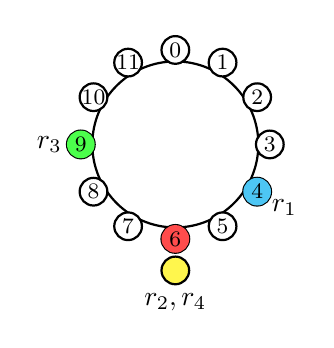
\begin{tikzpicture}[node distance =15em,>=stealth,->, thick] 
			\node[circle,minimum size =6em, draw, thick] (C){};
			\foreach \i in {0,...,11}\node[circle,minimum size
			=1em,draw,fill=white,thick]at(\i*30:1.2) (\i){};
			
			\node[circle,minimum size =1em,fill=cyan!70]at(11*30:1.2) (17){};
			\node[]at(11*30:1.6) (1721){{$r_1$}};
			\node[circle,minimum size =1em,fill=red!70]at(9*30:1.2) (18){}; 
			\node[circle,minimum size =1em,fill=yellow!70,draw,thick]at(9*30:1.6) (18){};
			\node[]at(9*30:2) (181){{$r_2,r_4$}}; 
			\node[circle,minimum size =1em,fill=green!70]at(6*30:1.2) (29){};
			\node[]at(6*30:1.6) (191){{$r_3$}}; 
			
			\foreach \i in {0,...,11}\node[circle,minimum size
			=1em]at(90 - \i*30:1.2) (pos){\footnotesize{\i}};

			\end{tikzpicture}
	}\hspace{-1em}
	\subfloat[][
	]{
			\centering 
			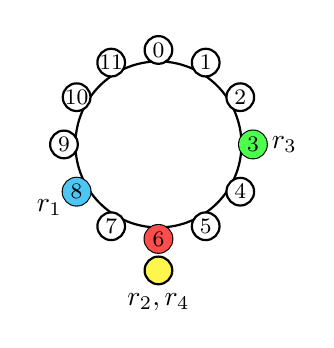
\begin{tikzpicture}[node distance =15em,>=stealth,->, thick] 
			\node[circle,minimum size =6em, draw, thick] (C){};
			\foreach \i in {0,...,11}\node[circle,minimum size
			=1em,draw,fill=white,thick]at(\i*30:1.2) (\i){};

			\node[circle,minimum size =1em,fill=cyan!70]at(7*30:1.2) (17){};
			\node[]at(7*30:1.6) (1721){{$r_1$}};
			\node[circle,minimum size =1em,fill=red!70]at(9*30:1.2) (18){}; 
			\node[circle,minimum size =1em,fill=yellow!70,draw,thick]at(9*30:1.6) (18){};
			\node[]at(9*30:2) (181){{$r_2,r_4$}};  
			\node[circle,minimum size =1em,fill=green!70]at(0*30:1.2) (29){};
			\node[]at(0*30:1.6) (191){{$r_3$}}; 
			
			\foreach \i in {0,...,11}\node[circle,minimum size
			=1em]at(90 - \i*30:1.2) (pos){\footnotesize{\i}};

			\end{tikzpicture}
	}\hspace{-1em}
	\subfloat[][
	]{
			\centering 
			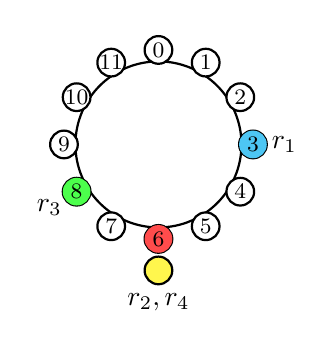
\begin{tikzpicture}[node distance =15em,>=stealth,->, thick] 
			\node[circle,minimum size =6em, draw, thick] (C){};
			\foreach \i in {0,...,11}\node[circle,minimum size
			=1em,draw,fill=white,thick]at(\i*30:1.2) (\i){};
			
			\node[circle,minimum size =1em,fill=green!70]at(7*30:1.2) (17){};
			\node[]at(7*30:1.6) (1721){{$r_3$}};
			\node[circle,minimum size =1em,fill=red!70]at(9*30:1.2) (18){}; 
			\node[circle,minimum size =1em,fill=yellow!70,draw,thick]at(9*30:1.6) (18){};
			\node[]at(9*30:2) (181){{$r_2,r_4$}}; 
			\node[circle,minimum size =1em,fill=cyan!70]at(0*30:1.2) (29){};
			\node[]at(0*30:1.6) (191){{$r_1$}}; 
			
			\foreach \i in {0,...,11}\node[circle,minimum size
			=1em]at(90 - \i*30:1.2) (pos){\footnotesize{\i}};

			\end{tikzpicture}
	}
	\caption{Equivalent configurations}
	\label{fig:confEq}
\end{figure}
\end{example}

\index{Symmetry}
A configuration is \emph{symmetrical} if there exists an axis of
symmetry that maps single robots to single robots, multiplicities
to multiplicities, and empty nodes to empty nodes.
\begin{definition}[Symmetries]
\label{def:ConfSym}
Configurations $c$ and $c'$ are \emph{symmetrical}, written $c \ \sym \ c'$, if there are some $m$ and $\beta$ such that $c' = \pi^m \circ \overline{\pi} \circ \pi^{-m} \circ c \circ \beta$, or $c' = \pi^{m+1} \circ \overline{\pi} \circ \pi^{-m} \circ c \circ \beta$\\
Configuration $c$ is \emph{symmetrical} if $c \ \sym \ c$.
\end{definition}
A symmetric configuration can be edge-edge\index{Symmetry!edge-edge symmetry}, node-edge\index{Symmetry!node-edge symmetry} or node-node\index{Symmetry!node-node symmetry} symmetrical if the axis goes through two edges, through one node and one edge, or through two nodes, respectively.
\begin{example}
\label{ex:confSym}
Configurations in Figure~\ref{fig:confSym} are symmetric.\\
%node-node sym
In configuration $a: a(r_1)=4$, $a(r_2)=6$, and $a(r_3)=8$, the axis of symmetry is the diameter that 
goes through the node $0$, and the node $6$. 
Let $\beta$ be the permutation defined by: $\beta(r_1) = r_3$, $\beta(r_3)=r_1$, and $\beta(r_2)=r_2$. 
The configuration $a$ is symmetrical since $a= \pi^6 \circ \overline{\pi} \circ \pi^{-6} \circ a \circ \beta$.\\
%node-edge sym
The configuration $b$ is symmetrical with an axis of symmetry that goes through the node $3$ and the edge $8-9$,
since $b = \pi^3 \circ \overline{\pi} \circ \pi^{-3} \circ b \circ \beta$, where $\beta$ is the robot permutation
defined by: $\beta(r_1)=r_3$, $\beta(r_3)=r_1$, $\beta(r_2)=r_4$, and $\beta(r_4)=r_2$.\\
%edge-edge sym
The configuration $c$ is symmetrical with an axis of symmetry that goes through the edges $2-3$ and $7-8$, 
since $c = \pi^3 \circ \overline{\pi} \circ \pi^{-2} \circ c \circ \beta$, where $\beta$ is the robot permutation
defined by: $\beta(r_1)=r_3$, $\beta(r_3)=r_1$, $\beta(r_2)=r_4$, and $\beta(r_4)=r_2$.\\
\begin{figure} % robot tous du même gris
\centering
\subfloat[][: node-node
	]{
			\centering 
			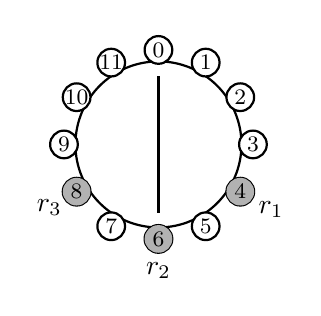
\begin{tikzpicture}[node distance =15em,>=stealth, thick] 
			\node[circle,minimum size =6em, draw, thick] (C){};
			\foreach \i in {0,...,11}\node[circle,minimum size
			=1em,draw,fill=white,thick]at(\i*30:1.2) (\i){};
					
			\node[circle,minimum size =1em,fill=gray!60]at(11*30:1.2) (17){};
			\node[]at(11*30:1.65) (1721){{$r_1$}};
			\node[circle,minimum size =1em,fill=gray!60]at(9*30:1.2) (18){};
			\node[]at(9*30:1.6) (181){{$r_2$}}; 
			\node[circle,minimum size =1em,fill=gray!60]at(7*30:1.2) (29){};
			\node[]at(7*30:1.6) (191){{$r_3$}}; 
			%\node[circle,minimum size =1em,fill=gray!60]at(3*30:1.2) (29){};
			%\node[]at(3*30:1.6) (191){{$r_4$}}; 
			
			\node[]at(90 - 0*30:1.0) (i){};
			\node[]at(90 - 6*30:1.0) (ii){};
			\draw (i) -- (ii);
						
			\foreach \i in {0,...,11}\node[circle,minimum size
			=1em]at(90 - \i*30:1.2) (pos){\footnotesize{\i}};

			\end{tikzpicture}
	}\hspace{-0.3em}
	\subfloat[][: node-edge
	]{
			\centering 
			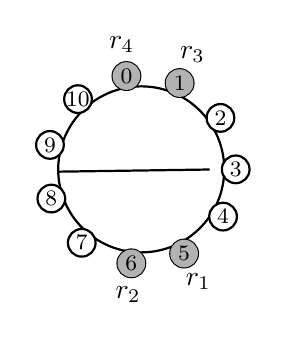
\begin{tikzpicture}[node distance =15em,>=stealth, thick] 
			\node[circle,minimum size =6em, draw, thick] (C){};
			\foreach \i in {0,...,10}\node[circle,minimum size
			=1em,draw,fill=white,thick]at(\i*33:1.2) (\i){};
			\node[circle,minimum size =1em,fill=gray!60]at(9*33:1.2) (17){};
			\node[]at(9*33:1.6) (1721){{$r_1$}};
			\node[circle,minimum size =1em,fill=gray!60]at(8*33:1.2) (17){};
			\node[]at(8*33:1.6) (1721){{$r_2$}};
			\node[circle,minimum size =1em,fill=gray!60]at(2*33:1.2) (18){}; 
			\node[]at(2*33:1.6) (181){{$r_3$}}; 
			\node[circle,minimum size =1em,fill=gray!60]at(3*33:1.2) (29){};
			\node[]at(3*33:1.6) (191){{$r_4$}}; 
			
			\node[]at(99 - 3*33:1.0) (i){};
			\node[]at(102 - 8.5*33:1.2) (ii){};
			\draw (i) -- (ii);
			
			\foreach \i in {0,...,3}\node[circle,minimum size
			=1em]at(-\i*33+99:1.2) (pos){\footnotesize{\i}};
			\foreach \i in {4,...,9}\node[circle,minimum size
			=1em]at(-\i*33+102:1.2) (pos){\footnotesize{\i}};
			\node[circle,minimum size
			=1em]at(102 - 10*33:1.2) (pos){\footnotesize{10}};

			\end{tikzpicture}
	}\hspace{0.3em}
	\subfloat[][: edge-edge
	]{
			\centering 
			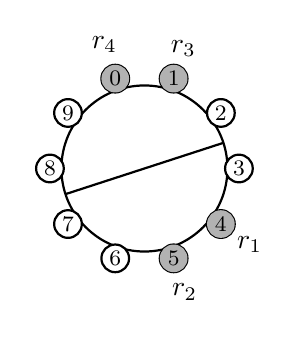
\begin{tikzpicture}[node distance =15em,>=stealth, thick] 
			\node[circle,minimum size =6em, draw, thick] (C){};
			\foreach \i in {0,...,9}\node[circle,minimum size
			=1em,draw,fill=white,thick]at(\i*36:1.2) (\i){};
			\node[circle,minimum size =1em,fill=gray!60]at(9*36:1.2) (17){};
			\node[]at(9*36:1.65) (1721){{$r_1$}};
			\node[circle,minimum size =1em,fill=gray!60]at(8*36:1.2) (17){};
			\node[]at(8*36:1.65) (1721){{$r_2$}};
			\node[circle,minimum size =1em,fill=gray!60]at(2*36:1.2) (18){}; 
			\node[]at(2*36:1.6) (181){{$r_3$}}; 
			\node[circle,minimum size =1em,fill=gray!60]at(3*36:1.2) (29){};
			\node[]at(3*36:1.65) (191){{$r_4$}}; 
			
			\node[]at(108 - 2.5*36:1.2) (i){};
			\node[]at(108 - 7.5*36:1.2) (ii){};
			\draw (i) -- (ii);
			
			\foreach \i in {0,...,9}\node[circle,minimum size
			=1em]at(108 - \i*36:1.2) (pos){\footnotesize{\i}};

			\end{tikzpicture}
	}
	\caption{Symmetrical configurations}
	\label{fig:confSym}
\end{figure}
\end{example}

When a configuration presents several axes of symmetry, the configuration is periodic: it means that the
configuration is invariant by non-trivial rotation $\ie$ a permutation $\pi^m$ for some $m \in \N$.
A configuration can be periodic without axis of symmetry, moreover
we call a configuration that is neither periodic nor symmetrical nor contains a tower
a \emph{rigid}\index{rigid} configuration.
Note that a symmetric configuration is not periodic if and only if it has exactly one axis of symmetry, 
and that a periodic configuration only occurs when $n$ and $k$ are not coprime.
\begin{example}
The configuration $a$ is \emph{periodic} due to several axes of symmetry.
The configuration $b$  is periodic but does not contain any axis of symmetry.
The configuration $c$ is rigid.
\begin{figure}[h] % robot tous du même gris
\centering
	\subfloat[][: periodical
	]{
			\centering 
			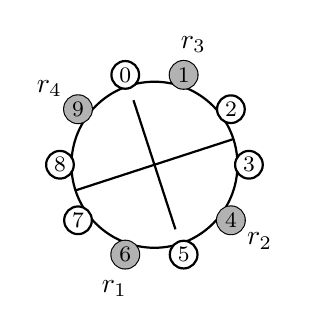
\begin{tikzpicture}[node distance =15em,>=stealth, thick] 
			\node[circle,minimum size =6em, draw, thick] (C){};
			\foreach \i in {0,...,9}\node[circle,minimum size
			=1em,draw,fill=white,thick]at(\i*36:1.2) (\i){};
			\node[circle,minimum size =1em,fill=gray!60]at(7*36:1.2) (17){};
			\node[]at(7*36:1.65) (1721){{$r_1$}};
			\node[circle,minimum size =1em,fill=gray!60]at(9*36:1.2) (17){};
			\node[]at(9*36:1.65) (1721){{$r_2$}};
			\node[circle,minimum size =1em,fill=gray!60]at(2*36:1.2) (18){}; 
			\node[]at(2*36:1.6) (181){{$r_3$}}; 
			\node[circle,minimum size =1em,fill=gray!60]at(4*36:1.2) (29){};
			\node[]at(4*36:1.65) (191){{$r_4$}}; 
			
			\node[]at(108 - 2.5*36:1.2) (i){};
			\node[]at(108 - 7.5*36:1.2) (ii){};
			\draw (i) -- (ii);
			\node[]at(3*36:1.0) (3){};
			\node[]at(8*36:1.0) (8){};
			\draw (3) -- (8);
			
			\foreach \i in {0,...,9}\node[circle,minimum size
			=1em]at(108 - \i*36:1.2) (pos){\footnotesize{\i}};

			\end{tikzpicture}
	}\hspace{0.3em}
\subfloat[][: periodical
	]{
			\centering 
			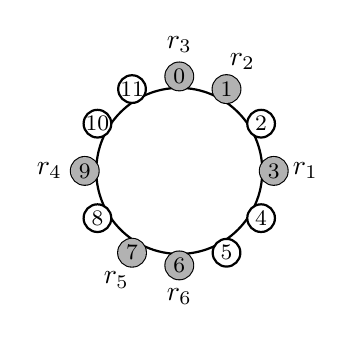
\begin{tikzpicture}[node distance =15em,>=stealth, thick] 
			\node[circle,minimum size =6em, draw, thick] (C){};
			\foreach \i in {0,...,11}\node[circle,minimum size
			=1em,draw,fill=white,thick]at(\i*30:1.2) (\i){};
			
			\node[circle,minimum size =1em,fill=gray!60]at(0*30:1.2) (17){};
			\node[]at(0*30:1.6) (1721){{$r_1$}};
			\node[circle,minimum size =1em,fill=gray!60]at(2*30:1.2) (17){};
			\node[]at(2*30:1.6) (1721){{$r_2$}};
			\node[circle,minimum size =1em,fill=gray!60]at(3*30:1.2) (17){};
			\node[]at(3*30:1.6) (1721){{$r_3$}};
			\node[circle,minimum size =1em,fill=gray!60]at(6*30:1.2) (29){};
			\node[]at(6*30:1.65) (191){{$r_4$}}; 
			\node[circle,minimum size =1em,fill=gray!60]at(8*30:1.2) (29){};
			\node[]at(8*30:1.6) (191){{$r_5$}}; 
			\node[circle,minimum size =1em,fill=gray!60]at(9*30:1.2) (29){};
			\node[]at(9*30:1.6) (191){{$r_6$}}; 
						
			\foreach \i in {0,...,11}\node[circle,minimum size
			=1em]at(90 - \i*30:1.2) (pos){\footnotesize{\i}};

			\end{tikzpicture}
	}\hspace{0.3em}
	\subfloat[][: rigid
	]{
			\centering 
			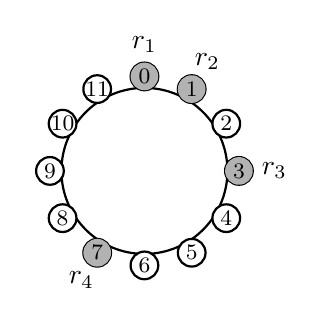
\begin{tikzpicture}[node distance =15em,>=stealth, thick] 
			\node[circle,minimum size =6em, draw, thick] (C){};
			\foreach \i in {0,...,11}\node[circle,minimum size
			=1em,draw,fill=white,thick]at(\i*30:1.2) (\i){};
					
			\node[circle,minimum size =1em,fill=gray!60]at(3*30:1.2) (17){};
			\node[]at(3*30:1.6) (1721){{$r_1$}};
			\node[circle,minimum size =1em,fill=gray!60]at(2*30:1.2) (29){};
			\node[]at(2*30:1.6) (191){{$r_2$}}; 
			\node[circle,minimum size =1em,fill=gray!60]at(0*30:1.2) (29){};
			\node[]at(0*30:1.65) (191){{$r_3$}}; 
			\node[circle,minimum size =1em,fill=gray!60]at(8*30:1.2) (29){};
			\node[]at(8*30:1.6) (191){{$r_4$}}; 
						
			\foreach \i in {0,...,11}\node[circle,minimum size
			=1em]at(90 - \i*30:1.2) (pos){\footnotesize{\i}};

			\end{tikzpicture}
	}
	\caption{Other types of configurations}
	\label{fig:otherConf}
\end{figure}

\end{example}

In a configuration, each robot can observe the entire ring, from
its own position. It takes a snapshot of this environment to compute its
future move. 

\subsection{Observations}\index{Observation}
\label{subsubsec:obs}
Since the robots have no chirality, they can
not distinguish the clockwise and the counter-clockwise direction. Since robots are anonymous, 
their observations can be described by a sequence of numbers, giving the free
nodes separating the robots, in a direction: We define $\mathcal{F}= \{(f_1,\cdots,f_k)
\mid \Sigma_{i=1}^k f_i=n-k, \ f_i\in \{-1,0,\cdots, n-1\} \}$. The two robots respectively positioned just 
before and just after some $f_i$ free nodes in a $k$-tuple $F$ are called \emph{consecutive robots}. 
When two consecutive robots occupy adjacent nodes,
$f_i=0$, and when these two robots occupy the same node, $f_i=-1$.
 For a $k$-tuple $F= (f_1,\cdots,f_k) \in \mathcal{F}$, we set
$\tilde{F} = (f_k, \cdots, f_1)$ the observation in the opposite
direction to $F$.  

\begin{definition}[Observations]
\label{def:obs}
The set of observations is $\Obs = \{ \{F, \tilde{F}\} | \ F \in \mathcal{F} \}$. 
\end{definition}
Note that when $F = \tilde{F}$, the corresponding observation is a
singleton. For an observation $o=\{(f_1,\cdots,f_k),(f_k, \cdots, f_1)\}$ in $\Obs$, 
we define the \emph{canonical configuration} by:
$c_o(r_1)=0$, $c_o(r_2)=f_1\plusN 1, \cdots, c_o(r_k) = \Sigma_{i=1}^k f_i
\plusN k$. Then $o$ is the observation of $r_1$ in $c_o$, also written
$obs(r_1,c_o)$. Note that $o$ is also the observation of $r_1$ in the
configuration $\overline{\pi} \circ c_o$ or in all configurations $c_o
\circ \beta$ for any permutation $\beta$ of $\Rob$ such that
$\beta(r_1)=r_1$ and in all configurations $\pi^m \circ c_o$ for any
$m$.

\begin{example}We illustrate this notion with examples from Figure~\ref{fig:confEq} and~\ref{fig:confSym}:\\
\label{ex:obs}
In Figure~\ref{fig:confEq}:
\begin{itemize}
\item $obs(r_1,a) = \{(1,-1,2,6),(6,2,-1,1)\} = \obs(r_1,b) = \obs(r_1,c)$,
\item $obs(r_2,a) = \{(-1,2,6,1),(1,6,2,-1)\} = \obs(r_2,b) = \obs(r_2,c) = \obs(r_2,d)$,
\item $obs(r_3,a) = \{(6,1,-1,2),(2,-1,1,6)\} = \obs(r_3,b) = \obs(r_3,c)$,
\item $obs(r_4,a) = \{(2,6,1,-1),(-1,1,6,2)\}= \obs(r_4,b) = \obs(r_4,c) = \obs(r_4,d)$.
\end{itemize}
As depicted in Figure~\ref{fig:confSym} when the configuration is
symmetrical with respect to a given axis, two ``corresponding" robots
on both sides of the axis have the same observation. For
simplification purpose we say that these robots are
symmetrical. Moreover if there is a single robot on the axis then its
observation is a singleton.
\begin{itemize}
\item $obs(r_1,a) = \{(1,1,7),(7,1,1)\} = \obs(r_3,a)$,
\item $obs(r_1,b) = \obs(r_3,b)$ and $obs(r_2,b) = \obs(r_4,b)$,
\item $obs(r_2,a) = \{(1,7,1)\}$.
\end{itemize}
\end{example}

We define on $\mathcal{F}$ the following relations:
\begin{itemize}
\item The rotation relation $\circlearrowright \subseteq \mathcal{F} \times \mathcal{F}$  defined by: for all  $F$, $F'\in \mathcal{F}$, $F \circlearrowright F'$ if and only if $F=(f_i,f_{i\plusK1}, \cdots, f_{i\plusK k-1})$ and $F'=(f_{i\plusK1}, f_{i\plusK2}, \cdots f_{i\plusK k})$.
%Since the robots have no chirality, one can easily observe that, for two configurations $C$ and $C'$, if $C=(d_1,\cdots, d_k)$ and $C'=(d_k, \cdots, d_1)$, then, for all robot $i$, $\obs_i(C)=\obs_i(C')$. 
\item The mirror relation  $\sim\subseteq \mathcal{F} \times \mathcal{F}$ defined by: for all  $F$, $F'\in \mathcal{F}$, $F\sim F'$
if and only if $F'=\tilde{F}$.
\end{itemize}

Combining the rotation relation and the mirror relation as  $(\circlearrowright\cup \sim)^*$ produces an equivalence relation on $\mathcal{F}:$ 
\begin{definition}[Equivalence on $\mathcal{F}$]
\label{def:obsEq}
 The equivalence relation ${\Oequiv}\subseteq \mathcal{F}\times\mathcal{F}$ is defined by ${\Oequiv} \stackrel{\mathrm{def}}{=} {(\circlearrowright\cup \sim)^*}$.
\end{definition}

We overload the relations $\circlearrowright$ and $\Oequiv$ on $\Obs$. Let the rotation relation on $\Obs$: $\circlearrowright \subseteq \Obs \times \Obs$ be defined for two observations $o$ and $o'$ by $o\circlearrowright o'$ if $o=\{F, \tilde{F}\}$, $o'=\{F',\tilde{F'}\}$, and $F \circlearrowright F'$.
Since $\Obs$ is closed by symmetry, the equivalence relation $\Oequiv$ on $\Obs$ can be reduced to the reflexive and transitive closure $\circlearrowright^*$ of $\circlearrowright$ on $\Obs$.
%For all $C\in \Config$, $\bigcup_{1\leq i\leq k} \obs(i,C) = \equivclass{\obs(?,C)}$.
%$\Oequiv\subseteq \Obs\times\Obs$.

%Let $\equivclass{o}$ be the equivalence class of an observation
%$o\in\Obs$. 
We define a mapping $\rep:{\ObsClass} \rightarrow
\Obs$, associating with each equivalence class a unique
representative:
%$\rep(\equivclass{o})\in \equivclass{o}$. 
Writing $\equivclass{o} = \{ \{F_1, \tilde{F_1}\}, \ldots, \{F_h, \tilde{F_h}\}\}$, 
we choose $F$ as the minimal $k$-tuple (wrt. the lexicographical order) in the subset 
$\{F_1, \tilde{F_1}, \ldots, F_h, \tilde{F_h}\}$ of $\mathcal{F}$. Then $\rep(\equivclass{o})= \{F, \tilde{F}\}$.

\smallskip The link between relation $\Cequiv$ on configurations and $\Oequiv$ is given by the following proposition: 
\begin{proposition}
\label{prop:Oequ}
For two configurations $c, c' \in \Config$, 
$c \Cequiv c' $ if and only if there exist $r, r' \in \Rob$ such that  $\obs(r,c)  \Oequiv \obs(r',c')$.
\end{proposition}
\begin{proof}~
Let $c$ and $c'$ be two configurations in $\Config$.\\
We first show that if
$c \Cequiv c'$  then there exist $r, r' \in \Rob$ such that $\obs(r,c)  \Oequiv \obs(r',c')$: 
	\begin{itemize}
		%[$\pi$: ]
		\item if $c' = \pi \circ c$ then $\forall r \in \Rob$, $\obs(r,c) = \obs(r, c')$.
		By induction  on $m$, we easily show that for $m \in \N$, if $c' = \pi^m \circ c$ then $\forall r \in \Rob~\obs(r,c) = \obs(r, c')$,
		%[$\overline{\pi}$: ] 
		\item if $c' = \overline{\pi} \circ c$ then $\forall r \in \Rob$, $\obs(r,c) = \obs(r, c')$,
		%[$\beta$: ]
		\item  if $c' = c \circ \beta$ for some robot permutation $\beta$, then $\forall r \in \Rob$, $\obs(r,c) = \obs(\beta(r),c')$.
	\end{itemize}
	This implies the desired result.

Conversely, we then show that if $\exists r,r' \in \Rob$  and $c,c' \in \Config$ 
such that $obs(r,c) \Oequiv \obs(r',c')$, then $c \Cequiv c'$.
If $obs(r,c) \Oequiv \obs(r',c')$, \textit{i.e., } $obs(r,c) \circlearrowright^* \obs(r',c')$, then there exists a permutation $\beta$
and $m \in \N$ such that $c' = \pi^m \circ c \circ \beta$ where $r' = \beta(r)$.
\end{proof}

Recall that robot decisions depend on their observations.  
Most of the time robots on the same tower have different observations (\textit{i.e.}, if they are not on an axis of symmetry), 
since they must have a similar behavior we introduce the notion of view.


\subsection{Views}\index{View}
\label{subsubsec:view}
In a given configuration, a robot view  depends on its observation.
With the following definition of view, two
robots on the same node have the same view.

\begin{definition}[View]
\label{def:view}  
The view of robot $r$ on a given configuration $c$ is defined from
$\obs(r,c)=\{(f_1,\cdots,f_k),(f_k, \cdots, f_1)\}$ by
$\view(r,c)=\{(f_i, \dots, f_j), (f_j,\dots, f_i)\}$, where $i<j$ are
respectively the smallest and greatest index such that $f_i\neq -1$
and $f_j\neq -1$. We denote by $\Views$ the set of all views.
 \end{definition}

\begin{example}~\\
\label{ex:sym-disoriented}
\begin{minipage}{0.7\textwidth}
Let $c$ be the configuration of Figure~\ref{fig:view}:
$$c(r_1)=1, c(r_2)=1,  c(r_3)=4,  c(r_4)=8, c(r_5)=8.$$
Observations of robot $r_4$ and robot $r_5$ are: 
\begin{itemize}
\item $obs(r_4,c) = \{(-1,2,-1,2,3),(3,2,-1,2,-1)\} $, 
\item $obs(r_5,c) = \{(2,-1,2,3,-1),(-1,3,2,-1,2)\}$.
\end{itemize}
\end{minipage}\hspace{1em}
\begin{minipage}{0.25\textwidth}
			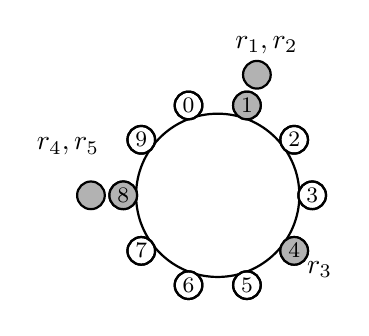
\begin{tikzpicture}[node distance =15em,>=stealth, thick] 
			\node[circle,minimum size =5.9em, draw, thick] (C){};
			\foreach \i in {0,...,9}\node[circle,minimum size
			=1em,draw,fill=white,thick]at(\i*36:1.2) (\i){};
			\node[circle,minimum size =1em,fill=gray!60]at(9*36:1.2) (17){};
			\node[]at(9*36:1.6) (1721){{$r_3$}};
			\node[circle,minimum size =1em,fill=gray!60]at(2*36:1.2) (18){};
			\node[circle,minimum size =1em,fill=gray!60]at(2*36:1.61) (29){};
			\node[]at(2*36:2) (181){{$r_1, r_2$}}; 
			\node[circle,minimum size =1em,fill=gray!60]at(5*36:1.2) (29){};
			\node[circle,minimum size =1em,fill=gray!60]at(5*36:1.61) (29){};
			\node[]at(4.5*36:2) (191){{$r_4, r_5$}}; 
			
			\foreach \i in {0,...,9}\node[circle,minimum size
			=1em]at(108 - \i*36:1.2) (pos){\footnotesize{\i}};
			\node[circle,minimum size=1em,draw,thick]at(5*36:1.61) (bla){};
			\node[circle,minimum size=1em,draw,thick]at(2*36:1.61) (bli){};
			\foreach \i in {0,...,9}\node[circle,minimum size
			=1em,draw,thick]at(\i*36:1.2) (\i){};
			
			\end{tikzpicture}
			\captionof{figure}{View}
			\label{fig:view}
\end{minipage}\\
and their views are $\view(r_4,c)=\view(r_5,c)=\{(2,-1,2,3),(3,2,-1,2)\}$.\\
\end{example}
Note that if a robot does not belong to a tower then its view is equal
to its observation. For instance in figure~\ref{fig:view}, we have $obs(r_3,c) =
\view(r_3,c)$.  Moreover when a tower is on an axis of symmetry, the views of the robots 
on this tower are singletons. Hence, using views instead of observations, the view of any
robot on an axis of symmetry is a singleton: such robots 
are called \emph{disoriented}  because they cannot distinguish one 
direction from the other. 
%todo index disoriented


Ordering the tuples of the form $(f_i,\dots,f_j)$ by lexicographical
order, we can obtain from a view of a robot $r$ the maximal and the minimal view,
denoted respectively by $\view^{\max\_r}$ and $\view^{\min\_r}$.

A view can also be described by what we call an
$F$-$R$-$T$ sequence: an alternating sequence of symbols $F$, $R$ and
$T$ indexed by natural numbers: $F_x$ stands for $x$ consecutive free
nodes, $R_x$ for $x$ consecutive nodes, each one occupied by a single
robot, and $T_x$ for a tower of $x$ robots.

We represent a class of configurations thanks to the minimal view,
written as a $F$-$R$-$T$ sequence. In the sequel, when describing 
a configuration (class), we simply give the corresponding $F$-$R$-$T$ sequence.

\begin{example}View and $F$-$R$-$T$ sequence.\\
In Figure~\ref{fig:view}   					%prendre les examples pour r_4 
$obs(r_3,c)= \{(3,-1,2,-1,2),(2,-1,2,-1,3)\}$
is the observation of the robot $r_3$,
hence in this case 
\begin{itemize}
\item $\view^{\max\_r_3} = (3,-1,2,-1,2) = (R_1,F_3, T_2,F_2,T_2,F_2)$, 
\item $\view^{\min\_r_3} = (2,-1,2,-1,3) = (R_1, F_2, T_2,F_2,T_2,F_3)$.
\end{itemize}
The configuration class can be represented by: $(T_2,F_2,T_2,F_2,R_1,F_3)$
\end{example}


\subsection{Robot movements}
\label{subsub:move}
The possible movements along edges also depend on the graph shape. On
a ring there are only three possibilities: stay idle or move in
the clockwise or anti-clockwise direction. The state
``Ready to Move'' (depicted in Figure~\ref{fig:1}) is then divided
into three states $r.\clockwise$, $r.\counterclockwise$ and
$r.\still$. When a robot $r$ is in state $r.\clockwise$, it
means that it will shift to its neighboring node in the direction
given by $\view^{\max\_r}$.  Symmetrically, the robot in state
$r.\counterclockwise$ will go in the opposite direction.
We define $\overline{r.\clockwise} = r.\counterclockwise$, 			%example system state equivalence
$\overline{r.\counterclockwise} = r.\clockwise$, 
$\overline{r.\still} = r.\still$, and $ \overline{\RLC} = \RLC$.


\begin{figure}[h]
\centering 
\begin{tikzpicture} [thick, node distance= 10em,>=stealth,->, scale=0.8]
\node[ellipse, minimum width= 10em,minimum height=4em, draw] (RLC) [scale=0.8]{};
\node[text width=7em, initial, initial text={}, initial, text centered](RLC2){Ready to\\Look-Compute};

\node[ellipse,  minimum width=5em,minimum height=2em, draw,  below right = 5em and 3em of RLC](F){};
\node[text width=7em, text centered](F1)at(F){$r.\clockwise$};
\node[ellipse,  minimum width=5em,minimum height=2em, draw,below left = 5em and 3em of RLC](B){};
\node[text width=7em, text centered](B1)at(B){$r.\counterclockwise$};

\node[ellipse,  minimum width=5em,minimum height=2em, draw,  above = 4em of RLC](I){};
\node[text width=7em, text centered](I1)at(I){$r.\still$};

\path 	(RLC.south west)	edge[bend right] node[left,text centered]{$\counterclockwise$, $\?$} (B)
		(RLC.south east)	edge[bend left] node[right, text centered]{$\clockwise$, $\?$} (F)
		(B.north east)	edge[bend right] node[right]{\Move} (RLC.-140)
		(F.north west)	edge[bend left] node[left]{\Move} (RLC.-40)
		(I.230)	edge[bend right] node[left]{$\varepsilon$} (RLC.-240)
		(RLC.60)	edge[bend right] node[right]{\still} (I.-50);

\end{tikzpicture}
\caption{Automaton of robot $r$ on a ring.}
 \label{fig:ring}
\end{figure}

These movements, determined by the algorithm, are described by the
$\LC$ actions in the set $\Actions=\{ \clockwise,
\counterclockwise, \?, \still \}$. We define
$\overline{\clockwise}=\counterclockwise$,
$\overline{\counterclockwise}=\clockwise$, $\overline{\still}=\still$
and $\overline{\disoriented}=\disoriented$.

 For a given robot $r$, the choice of an
action depends on its own view of the configuration. 
If the robot chooses not to move, its action
is $\still$. If $\view^{\max\_r} \neq \view^{\min\_r}$, the
robot can choose between the two directions, producing actions
$\clockwise$ or $\counterclockwise$. Otherwise the action is $\?$,
corresponding to a non deterministic choice between $\clockwise$
and $\counterclockwise$.
This is depicted in Figure~\ref{fig:ring} which describes a robot
automaton for the case of the ring. 

This automaton will later be refined 
again, according to the algorithm executed by the robots. In particular, 
guards depending on the views will be associated with the actions, 
in order to implement a choice between them.


The equivalence between configurations can be extended to global states as follows.
We consider system states as pairs $(s,c)$, where the robot state $s$ is a mapping from 
$\Rob$ to $\{\Front, \Back, \Idle, \RLC \}$ and $c$ is a configuration. 
\begin{definition}\label{def:state-equiv}
Two system states $(s,c)$ and $(s',c')$ are equivalent 
if
%%%%%%%%%%%%%%%%A garder%%%%%%%%%%%%%%%%%%%%%%
%\begin{itemize}
%\item If $c'= \pi^{m} \circ \overline \pi \circ c \circ \beta$ for some $m$ and some robot permutation $\beta$, 
%then for any robot $r$, $s'(r)=\overline{ s(\beta(r))}$, 
%\item If $c'= \pi^{m} \circ c \circ \beta$  for some $m$ and some robot permutation $\beta$, 
%then for for any robot $r$, $s'(r)=s(\beta(r))$. 
%\end{itemize}
% en fait on a pas \overline car on donne toujours le mouvement en fonction de la vue du robot  et du coup ça ne change pas ... c'est en travaillant dans l'implémentation qu'on a besoin de l'overline car on donne toujours le sens des mouvements en foncions de la plus petite  des vues de la configuration 
\begin{itemize}
\item $c \Cequiv c'$,  if $c'= \overline \pi \circ \pi^{m} \circ  c \circ \beta$ or $c'= \pi^{m} \circ c \circ \beta$ 
 for some $m$ and some robot permutation $\beta$,
 \item  $s'(r)=s(\beta(r))$ for any robot $r$. 
 \end{itemize}
\end{definition}

\begin{example}
\label{ex:vpAsync}
This example illustrates the notion of equivalence of system states 
thanks to the system states $(s_a,a)$ and $(s_b,b)$ depicted in Figure~\ref{fig:ex:vpAsync}.
In this figure the robot states associated with the configurations $a$ and $b$ are respectively given by $s_a$, $s_b$ defined by:
$\mem_a(r_3) = \Front$, $\mem_a(r_1) = \Back = \mem_a(r_5)$, $\mem_a(r_2) = \RLC = \mem_a(r_4) = \mem_a(r_6) $, and 
$\mem_b(r_6) = \Front$, $\mem_b(r_2) = \Front = \mem_b(r_3)$, $\mem_b(r_1) = \RLC = \mem_b(r_4) = \mem_b(r_5)$.
The two configurations a and b are equivalent since there is robot permutation $\beta$ such that 
$a = \overline \pi \circ \pi^{-2} \circ b \circ \beta$ where $\beta$ is defined by: $\beta(r_1)= r_6$, $\beta(r_2)=r_5$,
$ \beta(r_3)=r_2$, $\beta(r_4)=r_4$, $ \beta(r_5)=r_3$, $ \beta(r_6)=r_1$.
The two system states are equivalent since $a \Cequiv b$ and $s_a(r_1) = s_b(\beta(r_2)) = \Back$, 
$s_a(r_2) = s_b(\beta(r_5)) = \RLC$, $s_a(r_3) = s_b(\beta(r_6)) = \Front$, $s_a(r_4) = s_b(\beta(r_4)) = \RLC$, 
$s_a(r_5) = s_b(\beta(r_3)) = \Back$, and $s_a(r_6) = s_b(\beta(r_1)) = \RLC$.

\begin{figure}[htbp]%n=12 k =6
\center
	\subfloat[][
	]{
			\centering 
			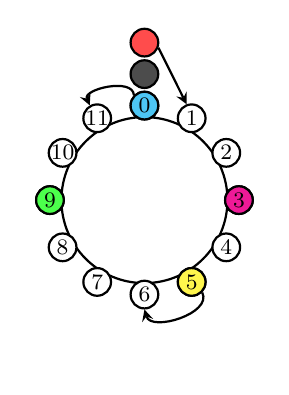
\begin{tikzpicture}[node distance =15em,>=stealth,->, thick] 
			\node[circle,minimum size =6em, draw, thick] (C){};
			\foreach \i in {0,...,11}\node[circle,minimum size
			=1em,draw,fill=white,thick]at(\i*30:1.2) (\i){};
			\node[circle,minimum size =1em,fill=cyan!70,draw,thick]at(3*30:1.2) (r1){};
			\node[circle,minimum size =1em,fill=black!70,draw,thick]at(3*30:1.6) (r2){};
			\node[circle,minimum size =1em,fill=red!70,draw,thick]at(3*30:2) (r3){};
			\node[circle,minimum size =1em,fill=magenta!90,draw,thick]at(0*30:1.2) (r4){}; 
			\node[circle,minimum size =1em,fill=yellow!70,draw,thick]at(10*30:1.2) (r5){}; 
			\node[circle,minimum size =1em,fill=green!70,draw,thick]at(6*30:1.2) (r6){};
						
			\foreach \i in {0,...,11}\node[circle,minimum size
			=1em]at(90 - \i*30:1.2) (pos){\footnotesize{\i}};
			\node[]at(9*30:2) (181){\large{$~$}}; 
			
			\path (r1.north west) edge[bend right=100,looseness=1, in=-80] (4.120);
			\path (r3.340) edge[] (2.110);
			\path (r5.south east) edge[bend left=100,looseness=1, in=90] (9.south);

			\end{tikzpicture}
	}\hspace{3em}
	\subfloat[][
	]{
\centering 
			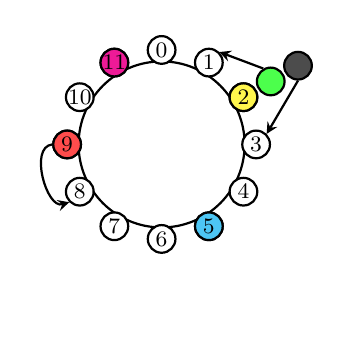
\begin{tikzpicture}[node distance =15em,>=stealth,->, thick] 
			\node[circle,minimum size =6em, draw, thick] (C){};
			\foreach \i in {0,...,11}\node[circle,minimum size
			=1em,draw,fill=white,thick]at(\i*30:1.2) (\i){};
			\node[circle,minimum size =1em,fill=yellow!70,draw,thick]at(1*30:1.2) (r1){};
			\node[circle,minimum size =1em,fill=green!70,draw,thick]at(1*30:1.6) (r2){};
			\node[circle,minimum size =1em,fill=black!70,draw,thick]at(1*30:2) (r3){};
			\node[circle,minimum size =1em,fill=cyan!70,draw,thick]at(10*30:1.2) (r4){}; 
			\node[circle,minimum size =1em,fill=red!70,draw,thick]at(6*30:1.2) (r5){}; 
			\node[circle,minimum size =1em,fill=magenta!90,draw,thick]at(4*30:1.2) (r6){};
						
			\foreach \i in {0,...,11}\node[circle,minimum size
			=1em]at(90 - \i*30:1.2) (pos){\footnotesize{\i}};
			\node[]at(9*30:2) (181){\large{$~$}}; 
			
			\path (r2.120) edge[] (2.north east);
			\path (r3.270) edge[] (0.45);
			\path (r5.west) edge[bend right=100,looseness=1, in=-90] (7.south west);
			
			\end{tikzpicture}
	}\hspace{2em}
	\captionsetup[subfloat]{labelformat=empty}
	\subfloat[Legend][
	]{
			\centering 
			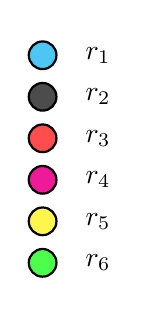
\begin{tikzpicture}[node distance =1.5em,>=stealth,->, thick] 
			\node[circle,minimum size =1em,draw,fill=cyan!70,thick] (1){};
			\node[circle,minimum size =1em,right of = 1,node distance =2em] (11){$r_1$};
			\node[circle,minimum size =1em,draw,fill=black!70,thick, below of = 1] (2){};
			\node[circle,minimum size =1em,right of = 2,node distance =2em] (21){$r_2$};
			\node[circle,minimum size =1em,draw,fill=red!70,thick, below of = 2] (3){};
			\node[circle,minimum size =1em,right of = 3,node distance =2em] (31){$r_3$};
			\node[circle,minimum size =1em,draw,fill=magenta!90,thick, below of = 3] (4){};
			\node[circle,minimum size =1em,right of = 4,node distance =2em] (41){$r_4$};
			\node[circle,minimum size =1em,draw,fill=yellow!70,thick, below of = 4] (5){};
			\node[circle,minimum size =1em,right of = 5,node distance =2em] (51){$r_5$};
			\node[circle,minimum size =1em,draw,fill=green!70,thick, below of = 5] (6){};
			\node[circle,minimum size =1em,right of = 6,node distance =2em] (61){$r_6$};
			\end{tikzpicture}
	}\caption{ %\begin{flushleft} 
	System configurations equivalence.}
	\label{fig:ex:vpAsync}
\end{figure}

The two system states $(a, s_a)$ and $(b, s_b)$ are equivalent, their configurations are in
 the class described by $T_3 F_2 R_1 F_1 R_1 F_3 R_1 F_2$ and the states satisfy:
\begin{itemize}%[noitemsep,topsep=0pt,parsep=0pt,partopsep=0pt]
\item Among the robots of the tower one wants to move $\clockwise$, one is in its $\RLC$ phase and the 
last one wants to move $\counterclockwise$.
\item The robot neighbor to $3$ free nodes
and $1$ free node wants to move in the direction of the $3$ free nodes.
\item All other robots are in their $\RLC$ phase.
\end{itemize}

\end{example}

\subsection{Robot algorithms}
The movements described above are defined by the algorithms. 
Recall  that a robot algorithm must ensure that: 
\begin{itemize}
\item A disoriented robot chooses a move in $\{\Idle, \?\}$ : either it stays idle or it plans a non deterministic move,
\item Two symmetrical robots plan the same move,
\item Robots on the same tower plan the same move.
\end{itemize}
By definition symmetrical robots have the same observation thus the same view, 
robots on the same tower have different observations but the same views.
Thus, an algorithm $\mathcal{S}$ can be given by a function that suggests a  
movement to a robot, according to its view. Such a function $\dec_\mathcal{S}:\Views\rightarrow \Actions$ 
is called a \emph{decision function} and defined as follows.

\begin{definition}[decision function] %%% f_C: \Views(C) ...
\label{def:decisionFunction}\index{Decision function}
A \emph{decision function} is a function $\dec:\Views\rightarrow \Actions$ such that, for $\view \in \Views$, if $|\view|=1$, then
$\dec(\view)\in\{\still,\disoriented\}$ and if $\dec(\view)=\disoriented$ then $|\view|=1$.
\end{definition}
This definition states that a disoriented robot $r$ in a configuration 
$c$, $\ie$ $|\view(r,c)|=1$ (see Example~\ref{ex:sym-disoriented}), cannot 
decide between $\clockwise$ and \counterclockwise.
Its possible moves are either $\Idle$ or \Doubt.
Conversely if the robot is not disoriented it has to decide,
hence its movement is not \Doubt. We write $\view \to \textit{action}$, when 
$\dec(\view)= \textit{action}$ and the function $\dec$ is clear from the context.  
A pair $\view \to \textit{action}$ is called a \emph{rule}.\index{rule}


\medskip To implement a given algorithm, we will need a pre-processing phase to express 
the corresponding rules in terms of guarded actions of the form $\emph{predicate} \rightarrow
\emph{action}$, where the predicate is evaluated on the robot view.
In the implementation, these rules are then translated into clockwise
or anti-clockwise moves, according to the current configuration.


Once the system is modeled, the requirements are expressed in \textsf{LTL}, and
model-checking is applied.

The next two chapters are devoted to case studies for the problems of
 ring exploration with stop and perpetual exclusive ring
exploration, with \cite{flocchini_computing_2007} and
\cite{blin_exclusive_2010} respectively, as representative protocols
of these two classes.

















